\documentclass[final]{fhnwreport}       %[mode] = draft or final
                                        %{class} = fhnwreport, article, 
                                        %          report, book, beamer, standalone
%%---Main Packages-----------------------------------------------------------------------
\usepackage[english, ngerman]{babel}	%Mul­tilin­gual sup­port for LaTeX
\usepackage[T1]{fontenc}				%Stan­dard pack­age for se­lect­ing font en­cod­ings
\usepackage[utf8]{inputenc}				%Ac­cept dif­fer­ent in­put en­cod­ings
\usepackage{lmodern}                    %The newer Font-Set
\usepackage{textcomp}					%LaTeX sup­port for the Text Com­pan­ion fonts
\usepackage{caption}					%Customising captions in floating environments
\usepackage{graphicx} 					%En­hanced sup­port for graph­ics
\usepackage{float}						%Im­proved in­ter­face for float­ing ob­jects
\usepackage{ifdraft}                    %Let you check if the doc is in draft mode

%%---Useful Packages---------------------------------------------------------------------
\usepackage{color}						%Colour control for LaTeX documents
\usepackage[pdftex,dvipsnames]{xcolor}  %Driver-in­de­pen­dent color ex­ten­sions for LaTeX
\usepackage{csquotes}                   %Simpler quoting with \enquote{}
\usepackage{siunitx} 					%A com­pre­hen­sive (SI) units pack­age
\usepackage{listings}					%Type­set source code list­ings us­ing LaTeX
\usepackage[bottom]{footmisc}			%A range of foot­note op­tions
\usepackage{footnote}					%Im­prove on LaTeX's foot­note han­dling
\usepackage{verbatim}					%Reim­ple­men­ta­tion of and ex­ten­sions to LaTeX ver­ba­tim
\usepackage[textsize=footnotesize]{todonotes} %Mark­ing things to do in a LaTeX doc­u­ment
\usepackage{titling}					%Control over the typesetting of the \maketitle command

%%---Tikz Packages-----------------------------------------------------------------------
\usepackage{standalone}
\usepackage{tikz}
\usepackage{circuitikz}
\usetikzlibrary{arrows}
\usetikzlibrary{calc}
\usetikzlibrary{intersections}

%%---Math Packages-----------------------------------------------------------------------
\usepackage{amsmath}					%AMS math­e­mat­i­cal fa­cil­i­ties for LaTeX
\usepackage{amssymb}					%Type­set­ting symbols (AMS style)
%\usepackage{amstext}
%\usepackage{amsfonts}
%\usepackage{breqn}
\usepackage{array}						%Ex­tend­ing the ar­ray and tab­u­lar en­vi­ron­ments
\usepackage{amsthm}					%Type­set­ting the­o­rems (AMS style)

%%---Table Packages----------------------------------------------------------------------
\usepackage{tabularx}					%Tab­u­lars with ad­justable-width columns
%\usepackage{longtable}
\usepackage{multirow}					%Create tab­u­lar cells span­ning mul­ti­ple rows
\usepackage{multicol}					%In­ter­mix sin­gle and mul­ti­ple columns

%%---PDF / Figure Packages---------------------------------------------------------------
\usepackage{pdfpages}					%In­clude PDF doc­u­ments in LaTeX
\usepackage{pdflscape}					%Make land­scape pages dis­play as land­scape
\usepackage{subfig}					    %Fig­ures di­vided into sub­fig­ures

%%---Other Packages----------------------------------------------------------------------
%\usepackage{xargs}                     %De­fine com­mands with many op­tional ar­gu­ments


%%---Bibliography------------------------------------------------------------------------
\usepackage[style=ieee,urldate=comp,backend=biber,language=english]{biblatex}
\addbibresource{literature/Kryg_Artikel.bib}

\DefineBibliographyStrings{ngerman}{
	url         = [Online]\addspace Available: ,
	urlseen		= {Abrufdatum}
}

%%---Main Settings-----------------------------------------------------------------------
\graphicspath{{./graphics/}}			%Defines the graphicspath
\geometry{twoside=false}				    %twoside=false disables the "bookstyle"
\setlength{\marginparwidth}{2cm}
\overfullrule=5em						%Creates a black rule if text goes over the margins => debugging




%%---User Definitions--------------------------------------------------------------------
%%Tabel-Definitions: (requires \usepackage{tabularx})
\newcolumntype{L}[1]{>{\raggedright\arraybackslash}p{#1}}    %column-width and alignment
\newcolumntype{C}[1]{>{\centering\arraybackslash}p{#1}}
\newcolumntype{R}[1]{>{\raggedleft\arraybackslash}p{#1}}

%%---Optional Package Settings-----------------------------------------------------------
%Listings-Settings: (requires \usepackage{listings}) => Example with Matlab Code
%\lstset{language=Matlab,%
%    basicstyle=\footnotesize\ttfamily,
%    breaklines=false,%
%    morekeywords={switch, case, otherwise},
%    keywordstyle=\color{Blue},%
%    tabsize=2,
%    %morekeywords=[2]{1}, keywordstyle=[2]{\color{black}},
%    identifierstyle=\color{Black},%
%    stringstyle=\color{Purple},
%    commentstyle=\color{Green},%
%    showstringspaces=false,%without this there will be a symbol in the places where there is a space
%    numbers=left,%
%    numberstyle={\tiny \color{black}},% size of the numbers
%    numbersep=9pt, % this defines how far the numbers are from the text
%    %emph=[1]{word1, word2,...},emphstyle=[1]\color{red}
%}							

% Eingefügt für C-Code Style
\renewcommand\lstlistingname{Codeausschnitt}
\lstset{language=C,
	basicstyle=\ttfamily,
	keywordstyle=\color{blue}\ttfamily,
	stringstyle=\color{red}\ttfamily,
	commentstyle=\color{green!70}\ttfamily,
	morecomment=[l][\color{magenta}]{\#}
}

%Hurenkinder und Schusterjungen verhindern (kein Scherz, Google es)
\clubpenalty10000
\widowpenalty10000
\displaywidowpenalty=10000	



%Titel mit Mathematik immer fett drucken
\usepackage{sectsty}
\allsectionsfont{\boldmath}




			                %loads all packages, definitions and settings											
\title{Benutzerhandbuch IoT-Raumautomation}  		        %Project Title
%\author{Team 1}      				    %Document Type => Technical Report, ...
%\date{\today}          				%Place and Date

\begin{document}

%%---TITLEPAGE---------------------------------------------------------------------------------
\thispagestyle{empty}
%	\ohead{\includegraphics[scale=0.5]{Bilder/Logo_FHNW.jpg}}
	\begin{figure}
		 \vspace*{-\topskip}\vspace*{-\headsep}
		
\includegraphics[scale=1]{graphics/fhnw_ht_logo_de.pdf}
	\end{figure}

	
	\begin{center}
		\vspace*{2cm}
		{\huge{\textbf{\thetitle}}}\\
		\vspace*{0.5cm}
		
	%	{\scshape\Large Artikel Kryptographie \\} 
		\Large{Windisch, \today}
		
		\vspace*{-1cm}						    %compensates the space after the date line.
		\vfill

		
	
		\vfill
		
		\begin{normalsize}
			{
			\renewcommand\arraystretch{2}
			\begin{tabular}{>{\bf}p{4cm} l}
			Autoren   		           & 	Gabriel Nussbaumer und Lukas Meienberger\\

			Hochschule                 &    Hochschule für Technik - FHNW\\
			Studiengang                &    Elektro- und Informationstechnik\\
%			Version                    &    1.0 %Normally not used!
			\end{tabular}
			}
		\end{normalsize}
	\end{center}
\clearpage
			
%%---ABSTRACT----------------------------------------------------------------------------
%\selectlanguage{english}				%ngerman or english
%\thispagestyle{empty}
%\begin{abstract}

Smart Home is the automation, and data-based control of electronic devices and light energy systems in your own home. This report is about a smart home system solution with MQTT communication. The development of an actor board with different switching possibilities, where electronic devices are connected, as well as the development of a touch sensor board with temperature measurement are described. A closed system with its own MQTT-broker is completed with the server software.The server software enables a perfect interaction between the components and the integration of a language assistant. The whole system can be integrated with existing Smart Home and offers cross-platform compatibility with other solutions.


%Der Softwareteil befasst sich mit verschiedenen Komponenten, so wird ein Framework für den Sensor/Aktorbaustein wie auch das Framework für den Inhouse Server und das MQTT Konzept beschrieben. Das Hardwarekonzept des Sensorbausteins besteht im wesentlichen aus einem WiFi fähigen Mikrocontroller, einem Temperatursensor, Buttons und LEDs. Dabei besteht der Sensorbaustein aus drei physisch getrennten Teilen: der Spannungsversorgung, dem Hauptprint und der Frontprint. Der Frontprint beinhaltet Touchsensoren und LEDs, welche einen individualisierten Einschaltzustand, z.B Lüftung ist an, signalisieren. Das wichtigste im Aktorbaustein ist ebenso ein Mikrocontroller mit WiFi, dazu kommen noch Relais, $10\;V$ Ein-/Ausgänge und LEDs, um den Schaltzustand der Relais zu signalisieren.

%Das Abstract ist eine Art Zusammenfassung des ganzen Dokuments. Es gibt einen Einblick in die Aufgabenstellung, wie diese umgesetzt wurde und welches Ergebnis erreicht wurde. Aus diesem Grund wird das Abstract immer ganz am Schluss der Arbeit verfasst. Es besteht aus einem zusammengehörenden Absatz und umfasst ungefähr 10 bis 20 Zeilen.Formeln, Referenzen oder andere Unterbrechungen haben im Text nichts zu suchen.Direkt unter dem Abstract folgt eine Liste von drei bis vier Stichworten/Keywords. Diese werden in alphabetischer Reihenfolge aufgelistet und beschreiben das Themengebiet der Arbeit.

%\vspace{2ex}
%\textbf{Keywords: Anleitung, LaTeX, Thesis, Vorlage}
\end{abstract}	


%%---TABLE OF CONTENTS-------------------------------------------------------------------
\pagenumbering{Roman}		
\selectlanguage{ngerman}				%ngerman or english
\tableofcontents
\clearpage

%%---TEXT--------------------------------------------------------------------------------
\pagenumbering{arabic}

\clearpage
\section{Installation Aktor}\label{sec:Aktor}
Das Aktor-Bord ist die physikalische Schnittstelle zu den Elektronischen Geräten. Die Relais K1 bis K4 können 250 Volt AC und 10 Ampere schalten. An den 0-10 Volt Ausgängen darf einen maximalen Strom von 4 mA bezogen werden.
\subsection{Anleitung einrichten}
\begin{figure}[H]
	\centering
	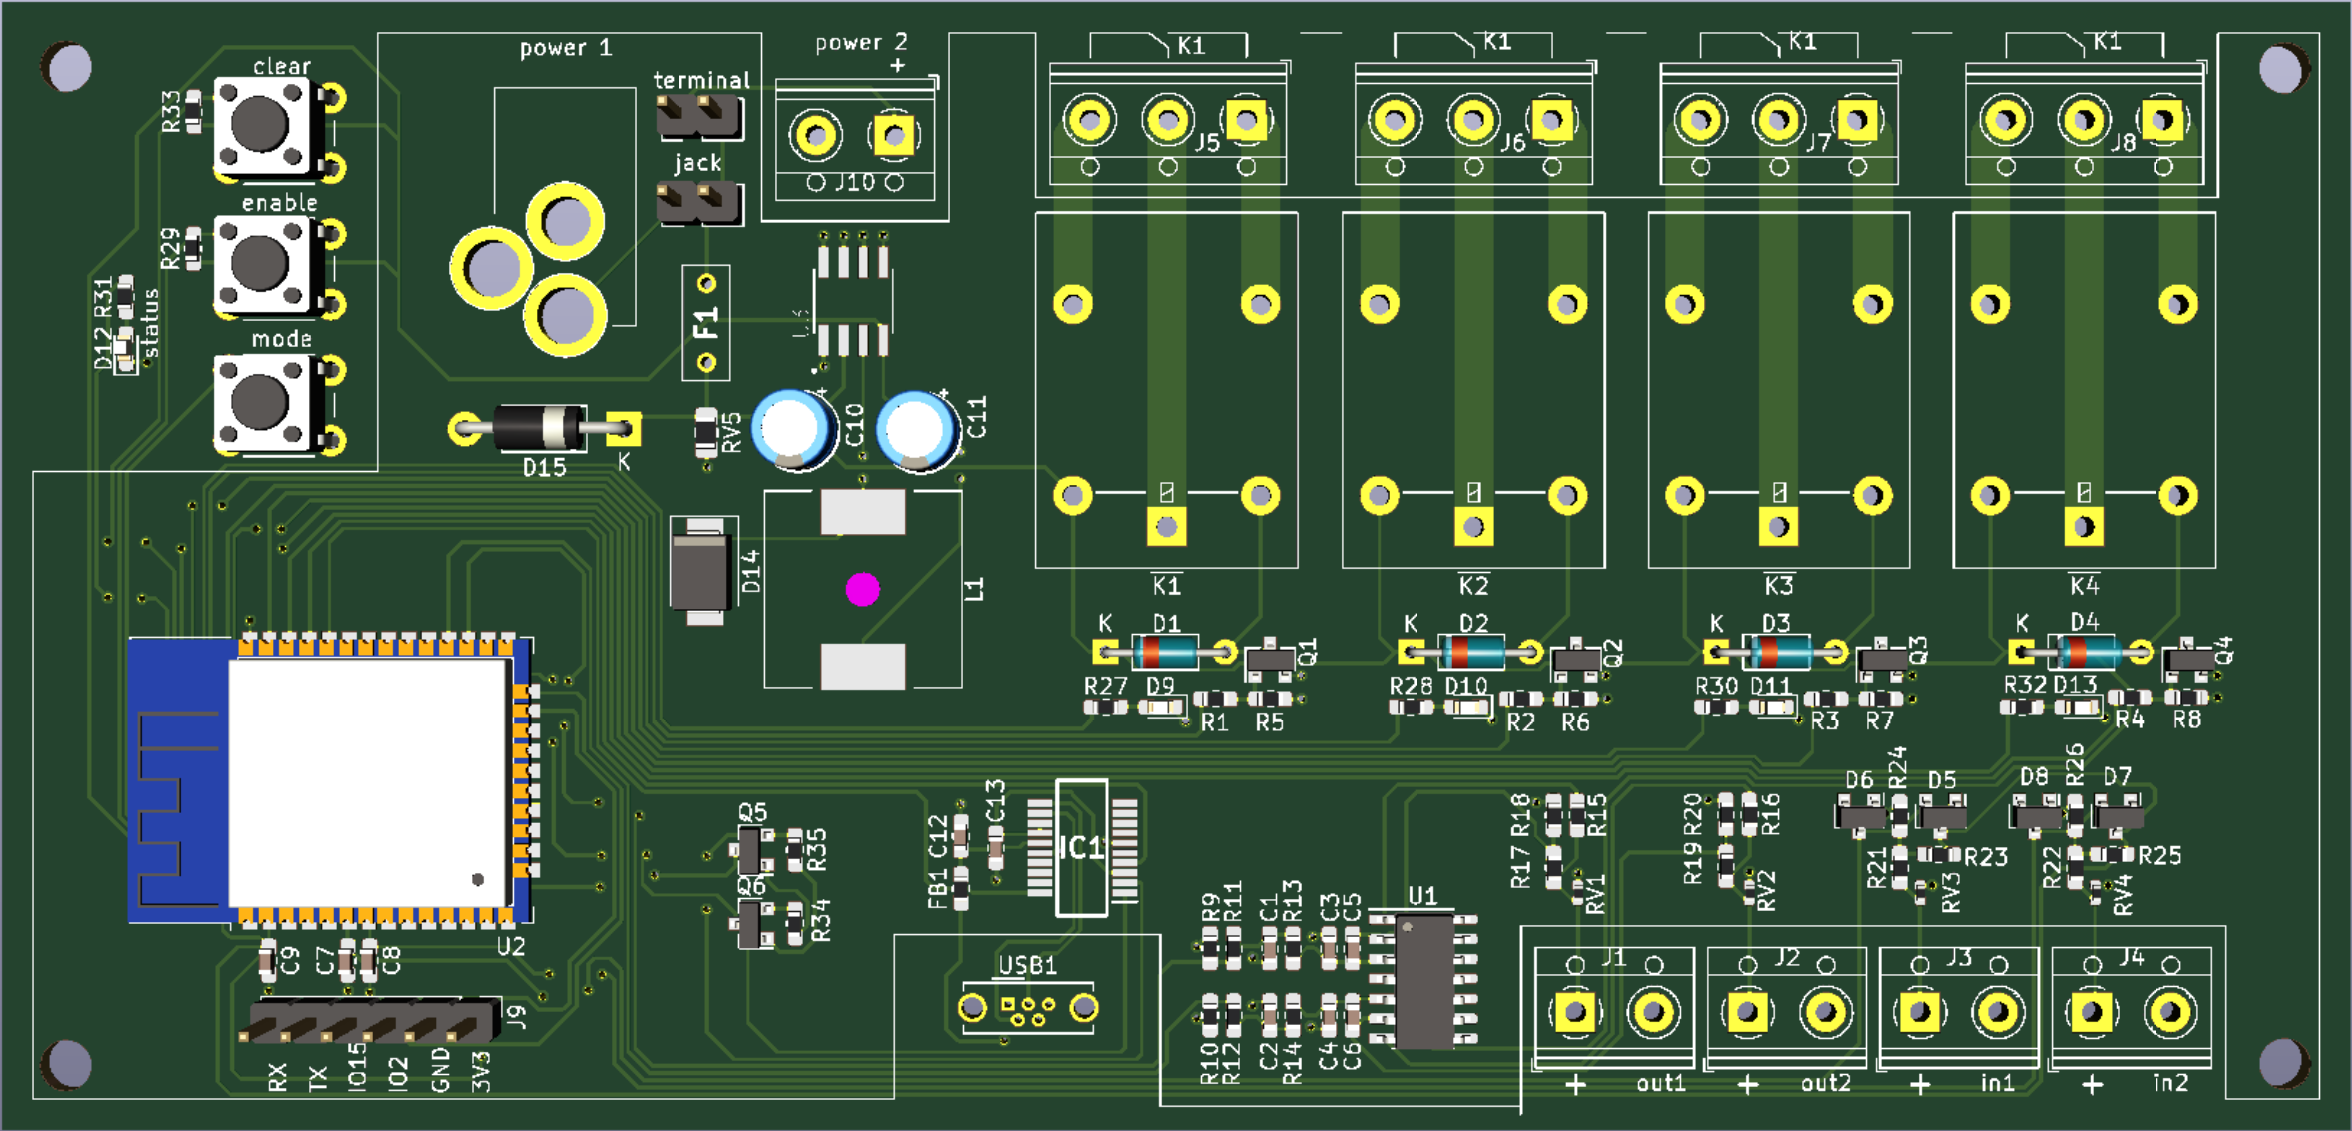
\includegraphics[width=\textwidth]{graphics/Aktorbaustein.png}
	\caption{Aktor Bord} 	
	\label{pic: OSGILayers}
\end{figure} 

\begin{enumerate}
	\item Das Gehäuse des Aktor-Bords, soll in eine Haupt- oder Unterverteilung eingebaut werden, wichtig ist zu beachten, dass sich dieser Standort innerhalb der eigenen WLAN-Reichweite befindet. Der Einbau ist im spannungslosen Zustand durchzuführen. \\
	\\
	\item Verbraucher wie Leuchten, Beschattungs-Systeme oder Ventilationen können in Schliesser- oder Öffnerbetrieb an den Relais K1 bis K4 angeschlossen werden. Wichtig ist zu beachten, dass die maximale Spannung von 250 Volt AC und maximaler Strom von 10 Ampere nicht überschritten wird.\\
		\\
	\item An den out1 und out2 Klemmen können Geräte mit einer 0-10 Volt Schnittstelle angeschlossen werden. Ein maximaler Strom von 4 mA darf nicht überschritten werden, damit die Spannung stabil bleibt.\\
	\\
	\item An den In1 und In2 Klemmen können 0-10 Volt Sensoren angeschlossen werden. Werden diese Eingänge nicht verwendet, wird eine Spannung von 0.25 V ermittelt. Falls 0 V gewünscht ist, kann der '+' Eingang auf Ground bzw. dem zweiten zweiten Anschluss der Klemme angeschlossen werden. \\
	\\
	\item Als Energieversorgung kann an den Power Klemmen eine 24 V DC Quelle angeschlossen werden. Das Board kann auch mit einem 24\,VDC Hohlstecker verbunden werden. Der Jumper muss entsprechend gesteckt werden, 'jack' für Hohlstecker oder "terminal" wenn die Speisung über Klemmen erfolgt. 
\end{enumerate}

\subsection{Inbetriebnahme}
Sobald das Aktor-Bord mit Spannung versorgt wird, startet der Mikrocontroller ein Access-Point und das Config-Portal des Bords. Mit einem beliebigen Gerät, kann nach einem WLAN-Netzwerk gesucht werden. Das Netzwerk hat den Namen 'Aktor' gefolgt von der 10 Stelligen Chip-ID des Mikrocontrollers. 
 
\begin{figure}[H]
	\begin{center}
	\begin{minipage}[b]{.3\linewidth} % [b] => Ausrichtung an \caption
		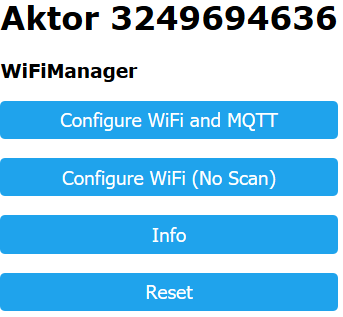
\includegraphics[width=\textwidth]{graphics/Configportal.PNG}
		\caption{Ansicht Configportal Frontseite}
	\end{minipage}
	\hspace{.1\linewidth}% Abstand zwischen Bilder
	\begin{minipage}[b]{.3\linewidth} % [b] => Ausrichtung an \caption
		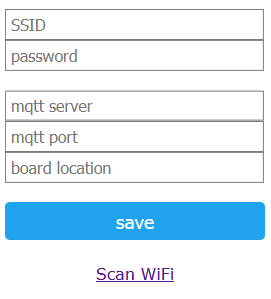
\includegraphics[width=\textwidth]{graphics/Configportal2.PNG}
		\caption{Parameter Config}
	\end{minipage}
\end{center}
\end{figure}
Mit der Funktion 'Scan WiFi' werden vorhanden Netzwerke angezeigt. Wird ein eigener MQTT Server installiert, kann an dieser Stelle die IP-Adresse angegeben werden, ansonsten der URL des öffentlichen MQTT-Broker. Der Port ist Default '1883' anzugeben. Die Eingabe bei 'board location' wird verwendet um MQTT-Topics zu generieren, sie muss also eindeutig sein und sollte keine Sonderzeichen beinhalten. Werden mehrere Aktor-Boards verbaut, unterscheiden sie sich an der 'bord location'. Mit der Taste 'save' werden die Eingaben gesichert und müssen bei einem erneuten Start nicht mehr eingegeben werden. Kann sich das Aktor Bord erfolgreich ins Lokale Netzwerk anmelden, blinkt die Status LED in einem regelmässigen Zyklus. Bei jeder Zustandsänderung der Statusleuchte wird eine Messung an den Eingängen In1 und In2 durchgeführt.

\subsection{Programmierung}
Verschiedene Eigenschaften können mit dem Entwicklertool zusätzlich verändert werden, wenn der Programmcode des Mikrocontrollers bearbeitet wird. In der nachfolgenden Tabelle sind Default-Konfigurationen enthalten.
\begin{table}[H]
\centering
\begin{tabular}{|l|l|l|}
	\hline 
	Bezeichnung & Variable & Wert \\ 
	\hline 
	Zeit Interwall Messungen & NUM\_SEC & 10 \\ 
	\hline 
	Allgemeiner MQTT-Topic  & MQTT\_SERIAL\_PUB & 'data/aktorboard/' \\ 
	\hline 
	Messungen für Mean Wert ADC & I & 100 \\ 
	\hline  
\end{tabular} 	
\end{table}
Werden schnelle Reaktionszeiten vom System verlangt, von Befehlseingabe bis zur Ausführung, können Funktionen direkt im Programmcode eingebunden werden. So kann eine Reaktionszeit von 300\,ms erreicht werden. In diesem Fall wird in der Funktion 'callback()' definiert, wenn topic 'data/sensorboard/location/s1' empfangen wird, wird Relais1 schalten.
\subsection{Netzwerkeinstellungen ändern}
Soll sich das Aktor-Board in ein anderes Netzwerk anmelden, gibt es zwei verschiedene Möglichkeiten die Einstellungen zu ändern. Falls während des Startvorgangs die 'Mode' Taste betätigt wird, öffnet der Mikrocontroller das Config-Portal. Das Config-Portal wird ebenfalls geöffnet, wenn das einst eingetragene Netzwerk nicht mehr gefunden wird und keine Verbindung hergestellt werden kann.
\subsection{System Tasten}
Mit der Taste 'enable' wird manuell ein Neustart durchgeführt. \\
Mit der Taste 'mode' wird das Config-Portal eröffnet die Taste muss beim Startvorgang mindestens 5\,s Betätigt werden.\\
Die Taste 'clear' hat auf dem Prototyp Aktor-Board keine Funktion.

\subsection{Topics}
In der Nachfolgenden Tabelle sind die automatisch generierten Topics, welche weiter in Openhab verwendet werden, um festzulegen welches Relais bei welchem Befehl schaltet. Als 'location' wurde im Config-Portal in diesem Fall 'location' eingetragen.
\begin{table}[H]
	\centering
	\begin{tabular}{|l|l|}
		\hline 
		 Topic  & Funktion  \\ 
		\hline 
		data/aktorboard/location/K1 & Schaltet Relais 1  \\ 
		\hline
		data/aktorboard/location/K2 & Schaltet Relais 2  \\ 
		\hline
		data/aktorboard/location/K3 & Schaltet Relais 3  \\ 
		\hline
		data/aktorboard/location/K4 & Schaltet Relais 4  \\ 
		\hline 
		data/aktorboard/location/A1 & Schaltet 0-10V Output 1  \\ 
		\hline
		data/aktorboard/location/A2 & Schaltet 0-10V Output 2  \\ 
		\hline
		data/aktorboard/location/E1 & Publish 0-10V Input 1  \\ 
		\hline
		data/aktorboard/location/E2 & Publish 0-10V Input 2  \\ 
		\hline
	\end{tabular} 	
\caption{Generierte MQTT-Topics Aktor-Bord}
\label{tab: MQTT-Topics Aktor}
\end{table}
 
Mit den Topics werden die verschiedenen Anwendungen unterschieden, wobei sich der Zustand mit der Payload unterscheidet. Bei den Relais wird zwischen 'ON' und 'OFF' unterschieden. Bei den 0-10 Volt Inputs so wie Outputs enthält die Payload den entsprechenden Wert. 

\clearpage
\section{Installation Sensor}\label{sec:Sensor}

Das Sensor-Bord ist die Physikalische Schnittstelle, wo Actionen ausgelösst werden und anschliessend von Openhab empfangen und verarbeitet werden.
\subsection{Anleitung einrichten}
\begin{figure}[H]
	\begin{center}
		\begin{minipage}[b]{.3\linewidth} % [b] => Ausrichtung an \caption
			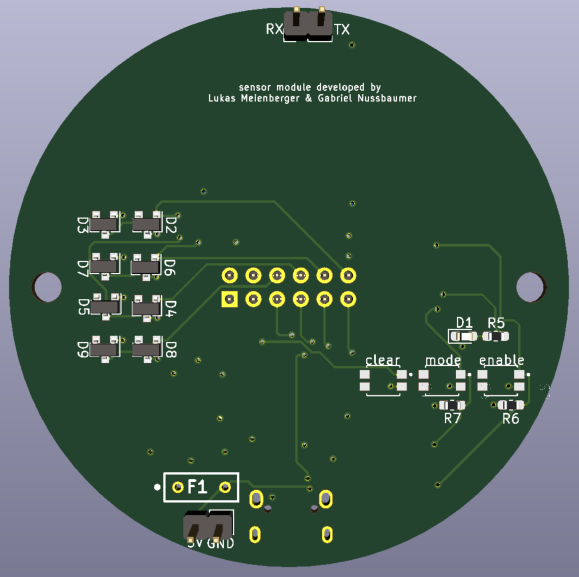
\includegraphics[width=\textwidth]{graphics/Sensor1.PNG}
			\caption{Sensor-Bord Rückseite}
		\end{minipage}
		\hspace{.1\linewidth}% Abstand zwischen Bilder
		\begin{minipage}[b]{.3\linewidth} % [b] => Ausrichtung an \caption
			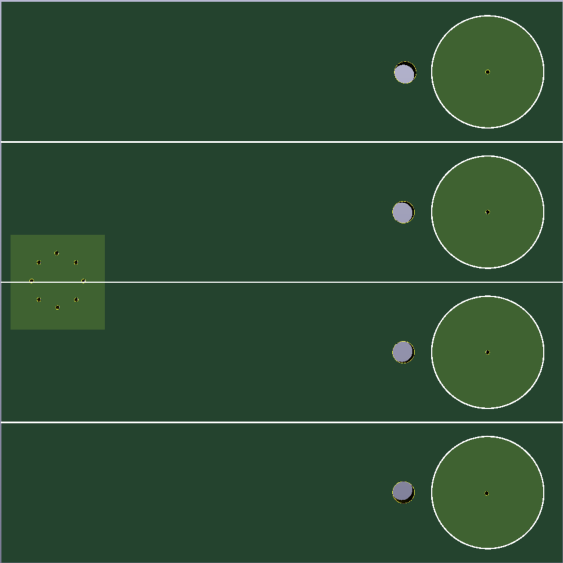
\includegraphics[width=\textwidth]{graphics/Sensor3.PNG}
			\caption{Frontprint}
		\end{minipage}
	\hspace{.1\linewidth}% Abstand zwischen Bilder
		\begin{minipage}[b]{.3\linewidth} % [b] => Ausrichtung an \caption
	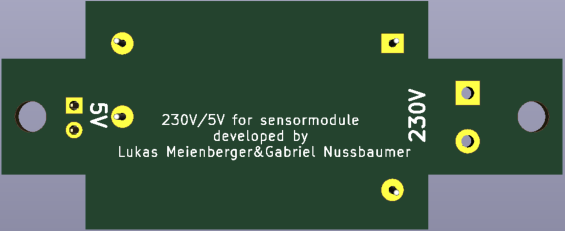
\includegraphics[width=\textwidth]{graphics/Sensor2.PNG}
	\caption{Spannungsversorgung Rückseite}
\end{minipage}
\end{center}
\end{figure}

\begin{enumerate}
	\item Die Installation ist in einem Spannungslosen Zustand durchzuführen.\\
	\\
	\item An der Rückseite vom der Spannungsversorgung wird die Netzspannung 230 V ADC angeschlossen\\
	\\
	\item Das Sensor-Bord wird zusammen gesteckt mit der Spannungsversorgung und mit einem Standart Feller Gr 1 Befestigungs Rahmen in eine Vorgesehene Einbauschalteröffnung eingebaut \\
	\\
	\item Der Frontplatte wird mit dem Abdeckrahmen Gr 1 auf das Sensor-Bord gesteckt. Die Beschriftung ist dringend zu Beachten.\\
	\\
	\end{enumerate}

\subsection{Inbetriebnahme}
Sobald das Sensor-Bord mit Spannung versorgt wird, startet das Configportal des Bords. Mit einem beliebigen Gerät kann im nach einem Wlan Netzwerk gesucht werden. Das Netzwerk hat den Namen "Sensor" gefolgt von der 10 Stelligen Chip-ID des Mikrocontrollers. 

Mit der Funktion Scan WiFi werden vorhanden Netzwerke angezeigt. Wird ein eigener MQTT Server installiert kann an dieser Stelle die IP Adresse angegeben der Port ist Default "1883". Die Eingabe bei "board location" wird verwendet um MQTT-Topics zu generieren, sie muss also eindeutig sein. Werden mehrere Sensor-Bords verbaut unterscheiden sie sich an der "bord location". Mit dem Button "save" werden die Eingaben gesichert un müssen bei einem erneuten Start nicht mehr eingegeben werden. Kann sich das Sensor-Bord erfolgreich ins Lokale Netzwerk anmelden, blinkt die Status Led in einem regelmässigen Zyklus. Bei jeder Zustandsänderung der Statusleuchte wird eine Temperatur Messung mit dem NTC-Widerstand durchgeführt. 

\subsection{Programmierung}
Verschiedene Eigenschaften können mit dem Entwicklertool zusätzlich verändert werden wenn der Programmcode des Mikrocontrollers bearbeitet wird. In der nachfolgenden Tabelle sind die wichtigsten Default-Konfigurationen enthalten.
\begin{table}[H]
	\centering
	\begin{tabular}{|l|l|l|}
		\hline 
		Bezeichnung & Variable & Wert \\ 
		\hline 
		Zeit Intervall Messungen & NUM\_SEC & 10 \\ 
		\hline 
		Allgemeiner MQTT-Topic  & MQTT\_SERIAL\_PUB& data/sensorboard/ \\ 
		\hline 
		Offset Temperatur Messung & b\_temp & 0.1369856 \\ 
		\hline  
		Steigung Temperatur Messung & m\_temp & 0.0008155002 \\ 
		\hline  
		Treshold Trigger Touchsensor & tresh& 15 \\ 
		\hline
		Messungen für Mean Wert Temperatur & I & 10 \\ 
		\hline  
		Messungen für Mean Wert Touchwert & count & 15 \\ 
		\hline  
	\end{tabular} 	
\end{table}
\subsection{Netzwerkeinstellungen ändern}
Soll sich das Sensor-Bord in ein anderes Netzwerk anmelden gibt es zwei verschiedenen Möglichkeiten. Wenn während des Startvorgangs die Clear Taste betätigt wird, eröffnet der Mikrocontroller das Config-Portal. Das Config-Portal wird ebenfalls geöffnet wenn das einst eingetragene Netzwerk nicht mehr erreichbar ist.

\subsection{Topics}
In Nachfolgenden Tabelle die generierten Topics, welche weiter in Openhab verwendet werden. Als location wurde im Config-Portal "location" eingetragen.
\begin{table}[H]
	\centering
	\begin{tabular}{|l|l|}
		\hline 
		Topic  & Funktion  \\ 
		\hline 
		data/sensorboard/location/S1 & Taster 1 wurde betätigt  \\ 
		\hline
		data/sensorboard/location/S2 & Taster 2 wurde betätigt  \\ 
		\hline
		data/sensorboard/location/S3 & Taster 3 wurde betätigt  \\ 
		\hline
		data/sensorboard/location/S4 & Taster 4 wurde betätigt  \\ 
		\hline
		data/sensorboard/location/S0 & Gemessene Raumtemperatur  \\ 
		\hline
			\end{tabular} 	
	\label{tab: MQTT-Topics Sensor}
	\caption{MQTT-Topics}
\end{table}


\section{OpenHab}
In dieser Arbeit wird als Server ein RaspberryPi verwendet. Als Software befindet sich Openhab auf dem Linux Betriebssystem vom RaspberryPi. Openhab ist eine Gebäudeautomation Software und bietet Kontabilität zwischen verschiedenen Smarthome Komponenten wie KNX, Sonos, oder Philips Hue. Der für das Projekt benötigte MQTT Brocker kann als Binding in Openhab eingebunden werden. Nach den Installationen kann der funktionserhalt mit den Geräten im selben lokalen Netzwerk gewährleistet werden, auch ohne Verbindung mit dem öffentlichen Internet.
\subsection{Archidektur}
OpenHab basiert auf der modularen OSGI Architektur.
\subsubsection{OSGI}
Die OSGI Technologie bietet eine Vielzahl  von dynamischen Spezifikationen für Java Systemkomponenten. Dies ermöglicht ein Entwicklungsmodell, bei dem eine Anwendung aus  mehreren Komponenten Entsteht die als Pakete gebündelt sind. Die Komponenten sind Bausteine und sind wiederverwendbar, sie kommunizieren lokal untereinander. Die OSGI Architektur ermöglicht es den Komponenten die Implementierung vor andern Komponenten zu verbergen, während Dienste kommunizieren über Objekte gerade wenn sie von anderen Komponenten gemeinsam genutzt werden. Dies reduziert die Gesamtkomplexität und ermöglicht eine hohe Zuverlässigkeit, da während laufendem System Wartung und Entwicklungsarbeiten Durchführt werden können.  

%quelle: https://www.openhab.org/v2.2/docs/developer/prerequisites/osgi.html#bundles

 \begin{figure}[H]
	\centering
	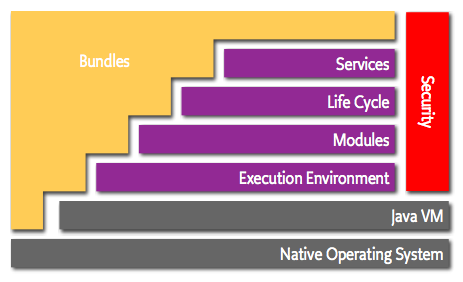
\includegraphics[width=\textwidth]{graphics/OSGI.png}
	\caption{OSGI Layers https://www.osgi.org/wp-content/uploads/layering-osgi.png} 	
	\label{pic: OSGILayers}
\end{figure} 

Bundles sind Module sie sind die kleinste Einheit der Modularisierung. Ein Bundle ist eine JAR-Datei mit zusätzlichen Meta-Informationen.\\
\\
In den Meta-Informationen sind Bundlesabhängigkeits Informationen. Ein Bundle kann von einem andern Bundel oder von einem Paket abhängig sein.\\
\\
Die OSGi-Runtime verwendet die Informationen über die Abhängigkeiten, um die Bundles zu verdrahten und versteckt alles in dieser JAR, sofern es nicht explizit exportiert wird. Die Abhängigkeiten zu den Java-Standardbibliotheken werden durch den Bundle-Header verwaltet, so dass es nicht notwendig ist, die Java-Kernpakete zu importieren.\\
\\
Bundles werden oft zur Registrierung und zum Konsum von Dienstleistungen verwendet.\\
\\
Die Bundles können in Laufzeit installiert, deinstalliert und geändert werden. Die Spezifikationen der OSGI Architektur also Abhängigkeiten und der Mechanismus wird mit Hilfe des Lebenszykluskonzepts erreicht. Der Rahmen führt verschiedene Zustände ein und regelt wie sich die vom Bundle exportierten Pakete und Dienste auswirken. 

 \begin{figure}[H]
	\centering
	\includegraphics[width=\textwidth]{graphics/BundleState.png}
	\caption{Bundle State Diagramm} 	
	\label{pic: BundleState}
\end{figure} 

In diesem Diagramm ist ersichtlich, dass Bundles während des Ausführens nicht geändert werden können, sonnst aber jederzeit.

\subsubsection{JAR}
\subsubsection{Übersicht Kommunikation Verbindungen}
Die Kommunikation zwischen den Komponenten geschieht mittels Event Bus. Alle nicht statusbezogenen Bundels informieren darüber andere Bundles über den Status von Events. Über diesen Bus Kommunizieren alle Binding mit einem phsikalischen Link zur realen Hardware. Mit dem Events werden auf asynchrone weise in diesem Bus veröffentlicht, durch den EventSubscriber definierte Callback-Schnittstellen werden diese zur entsprechender Funktion vorgesehenen Events wiederum Empfangen. Der EventSubsciber ist als OSGI Dienst registriert \cite{noauthor_event_nodate}.

https://www.openhab.org/docs/developer/utils/events.html
   
  \begin{figure}[H]
 	\centering
 	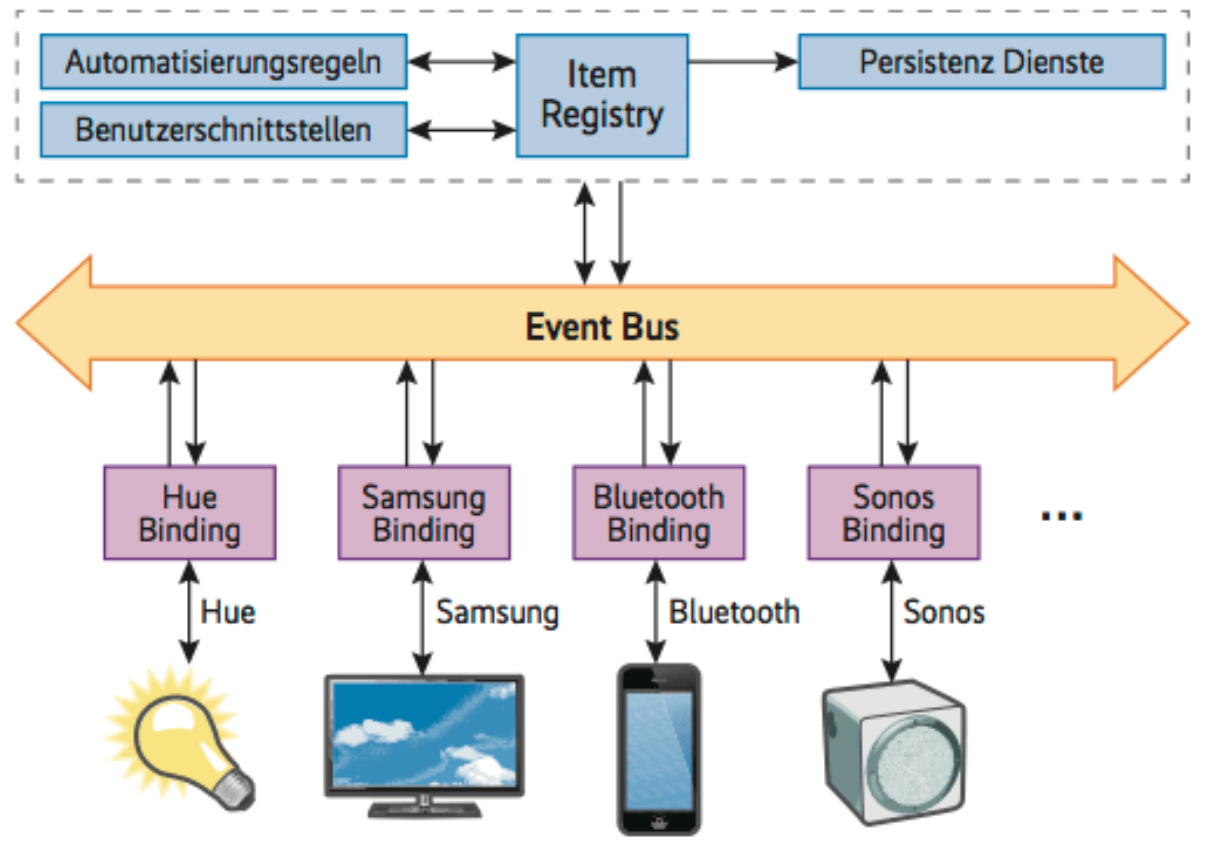
\includegraphics[width=\textwidth]{graphics/Eventbus.PNG}
 	\caption{Eventbus Openhab https://www.innoq.com/de/articles/2014/11/durchbruch/} 	
 	\label{pic: Eventbus}
 \end{figure} 
 
 In der Abbildung \ref{pic: Eventbus} ist der Eventbus dargestellt verschiedene Bindings mit Hardwarekomponenten von verschiedenen Smarthome lösungen empfange, die für sie vorgesehene Events
\clearpage
\section{Installation Sprach Assistant} \label{sec:Assistant}
Homeassitant ist die Schnittstelle, welche den Google Assitant mit Openhab verbindet. Die Kommunikation zwischen Homeassistant und Openhab findet über MQTT statt. Die Homeassistant Software wird auf ein weiteres Rasberrypi installiert.

\begin{enumerate}
	\item Download des Images für die Installation auf dem eigenen Raspi von der offiziellen Home Assistant \cite{assistant_installing_nodate}.
\item Micro SD Card flasen mit balenaEtcher \cite{noauthor_balenaetcher_nodate}. 
\item Mit ein USB Stick mit FAT32 formatieren und ihn als CONFIG benennen, ein Ordner mit dem Namen "network" erstellen, darin eine Text Datei erstellen, in der die Wlan Konfigurationen enthalten sind wie als Beipiel \cite{noauthor_home-assistantoperating-system_nodate} beschrieben oder in der Dokumentation enthalten.
\item USB Stick in und Micro SD Card mit Raspi verbinden und in Betrieb nehmen, dauert ca 20 min. Der USB Stick ist nur bei der ersten Inbetriebnahme notwendig.
\item Durch anwählen des Benutzernamen öffnet sich das Profil, Erweiterter Modus wählen.
\item Menupunkt Supervisor anwählen und in Add-on store File editor installieren, Start on boot und show in sidebar wählen
\item Mit File Editor Datei /config/configurationen.yaml bearbeiten: Mqtt-Message publish ermöglichen durch hinzufügen von Broker IP-Adresse und Port, siehe nachfolgende Abbildung.
\item Hinzu fügen von Schalter, welche mit Sprachbefehl Mqtt-Message generieren. Der Name des Schalters ist ebenso die Bezeichnung für den Sprachbefehl.
   \begin{figure}[H]
	\centering
	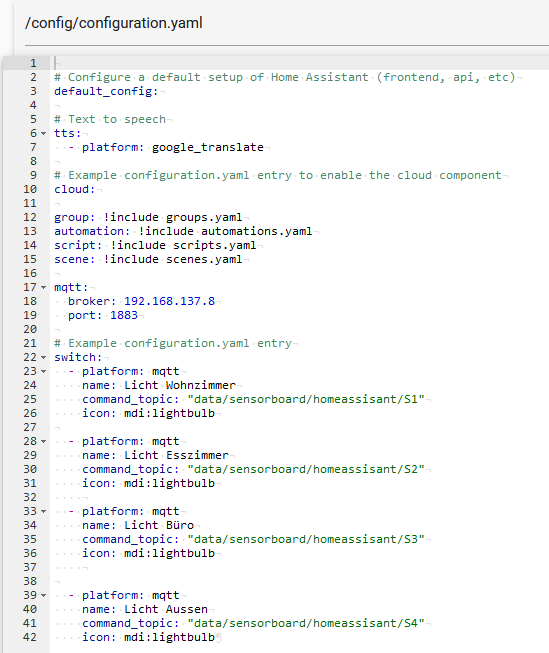
\includegraphics[width=0.75\textwidth]{graphics/Homeassostantconfig.PNG}
	\caption{Configfile Home Assistant} 	
	\label{pic: Configfile Home Assistant}
\end{figure}

 \item In den Einstellungen Home Assistant Cloud anmelden, Konto erstellen. Mit Google Home App  auf smartphone mit Gerät verbinden Home Assistant wählen und mit Cloud Benutzerkonto anmelden.
 
\end{enumerate}

\subsection{Topics}
In Nachfolgenden Tabelle sind die generierten Topics, welche weiter in Openhab verwendet werden.
\begin{table}[H]
	\centering
	\begin{tabular}{|l|l|}
		\hline 
		Topic  & Funktion  \\ 
		\hline 
	data/sensorboard/homeassisant/S1 & Sprachbefehl von Google Assistant empfangen  \\ 
		\hline
	data/sensorboard/homeassisant/S2 & Sprachbefehl von Google Assistant empfangen \\ 
		\hline
	data/sensorboard/homeassisant/S3 & Sprachbefehl von Google Assistant empfangen \\ 
		\hline
		data/sensorboard/homeassisant/S4 & Sprachbefehl von Google Assistant empfangen  \\ 
		\hline
	\end{tabular} 	
	\label{tab: MQTT-Topics Home Assistant}
	\caption{MQTT-Topics Home Assistant}
\end{table}
\section{Schluss}

\subsection{Reflektion}

In diesem Kapitel werden die Projekt Ziele Reflektiert. In der untenstehenden Tabelle \ref{tab: Teilziele} sind die zu beginn des Projekts Definierten Teilziele so wie der Status, in welchem der Fachbericht am ende verfasst wurde.
\begin{table}[h!]
	\small
	\begin{tabular}{|c|l|c|}
		\hline 
		Definition & Status \\ 
		\hline 
		Sensor- und Aktorbaustein sind als Prototypen hergestellt& Erfüllt \\ 
		\hline 
		Analyse und Evaluation Mikrocontroller & Erfüllt \\ 
		\hline 
		Frameware ist kompilierbar und erlaubt eine Inbetriebnahme der Prototypen & Erfüllt \\ 
		\hline 
		Signalverknüpfungen sind mit OpenHab realisierbar & Erfüllt \\ 
		\hline 
		Sensor- und Aktorbaustein sind optimiert (Redesign), Mechanisches Gehäuse ist erstellt  & Erfüllt \\ 
		\hline 
		Systemeinrichtung gestaltet sich Benutzerfreundlich & Erfüllt \\ 
		\hline 
		Validierung des gesamten Systems, Testergebnisse sind Dokumentiert n & Erfüllt \\ 
		\hline 
		Befehle können mit Sprachsteuerung ausgeführt werden & Erfüllt \\ 
		\hline 
		Dokumentation abgeschlossen & Erfüllt \\ 
		\hline 
		\end{tabular}
	\caption{Teilziele}
	\label{tab: Teilziele}	 
\end{table}



\subsubsection{Fazit}
 In diesem Projekt wurden Erfahrungen gewonnen, wie eine Hardware Lösung für eine IOT-Anwendung aussehen kann. Es gab einige Probleme wegen des verwendeten Mikrocontrollers, insbesondere des ADCs. Es wurde darauf verzichtet einen externen ADC zu verwenden und andere Lösungen gesucht, sowie die möglichen Verbesserungen der momentanen Lösung erarbeitet. Es hat sich darüber als schwierig herausgestellt, die Temperatur exakt zu messen, da die Umgebungsbedingungen anders sein können, wie stehende Luft und erwärmende Frontplatte. Weitere Erkenntnisse wurden ebenfalls im Bereich des Google Assistent gewonnen, durch die dynamische DNS Adresse  und SSL-Zertifikate gestaltete sich die Integration nicht mit einer direkten Verbindung, siehe Kapitel Sprachassistent.


\pagebreak


%\clearpage
%%---BIBLIOGRAPHY------------------------------------------------------------------------


{\sloppypar
%\printbibliography[heading=bibnumbered ]
\label{sec:lit}
\selectlanguage{ngerman}				%ngerman or english
\printbibliography
}

%\pagebreak

%\input{sections/8_0_Ehrlichkeitserklaerung}
%\pagebreak
%%---APPENDIX----------------------------------------------------------------------------
%\appendix
%\begin{appendix} %Anhang
	\section{Anhang Benutzerhandbuch}

%\includepdf[pages={1-2},nup=1x2,landscape=true,scale=0.85,offset=10 -40,pagecommand={\section{Eingefügtes Dokument; zwei Seiten auf einer}\label{app:Aufgabenstellung}\thispagestyle{myheadings}}]{appendix/aufgabenstellung.pdf} \newpage

%%Bei mehrseitigen Dokumenten die folgenden Seiten ohne Überschrift:
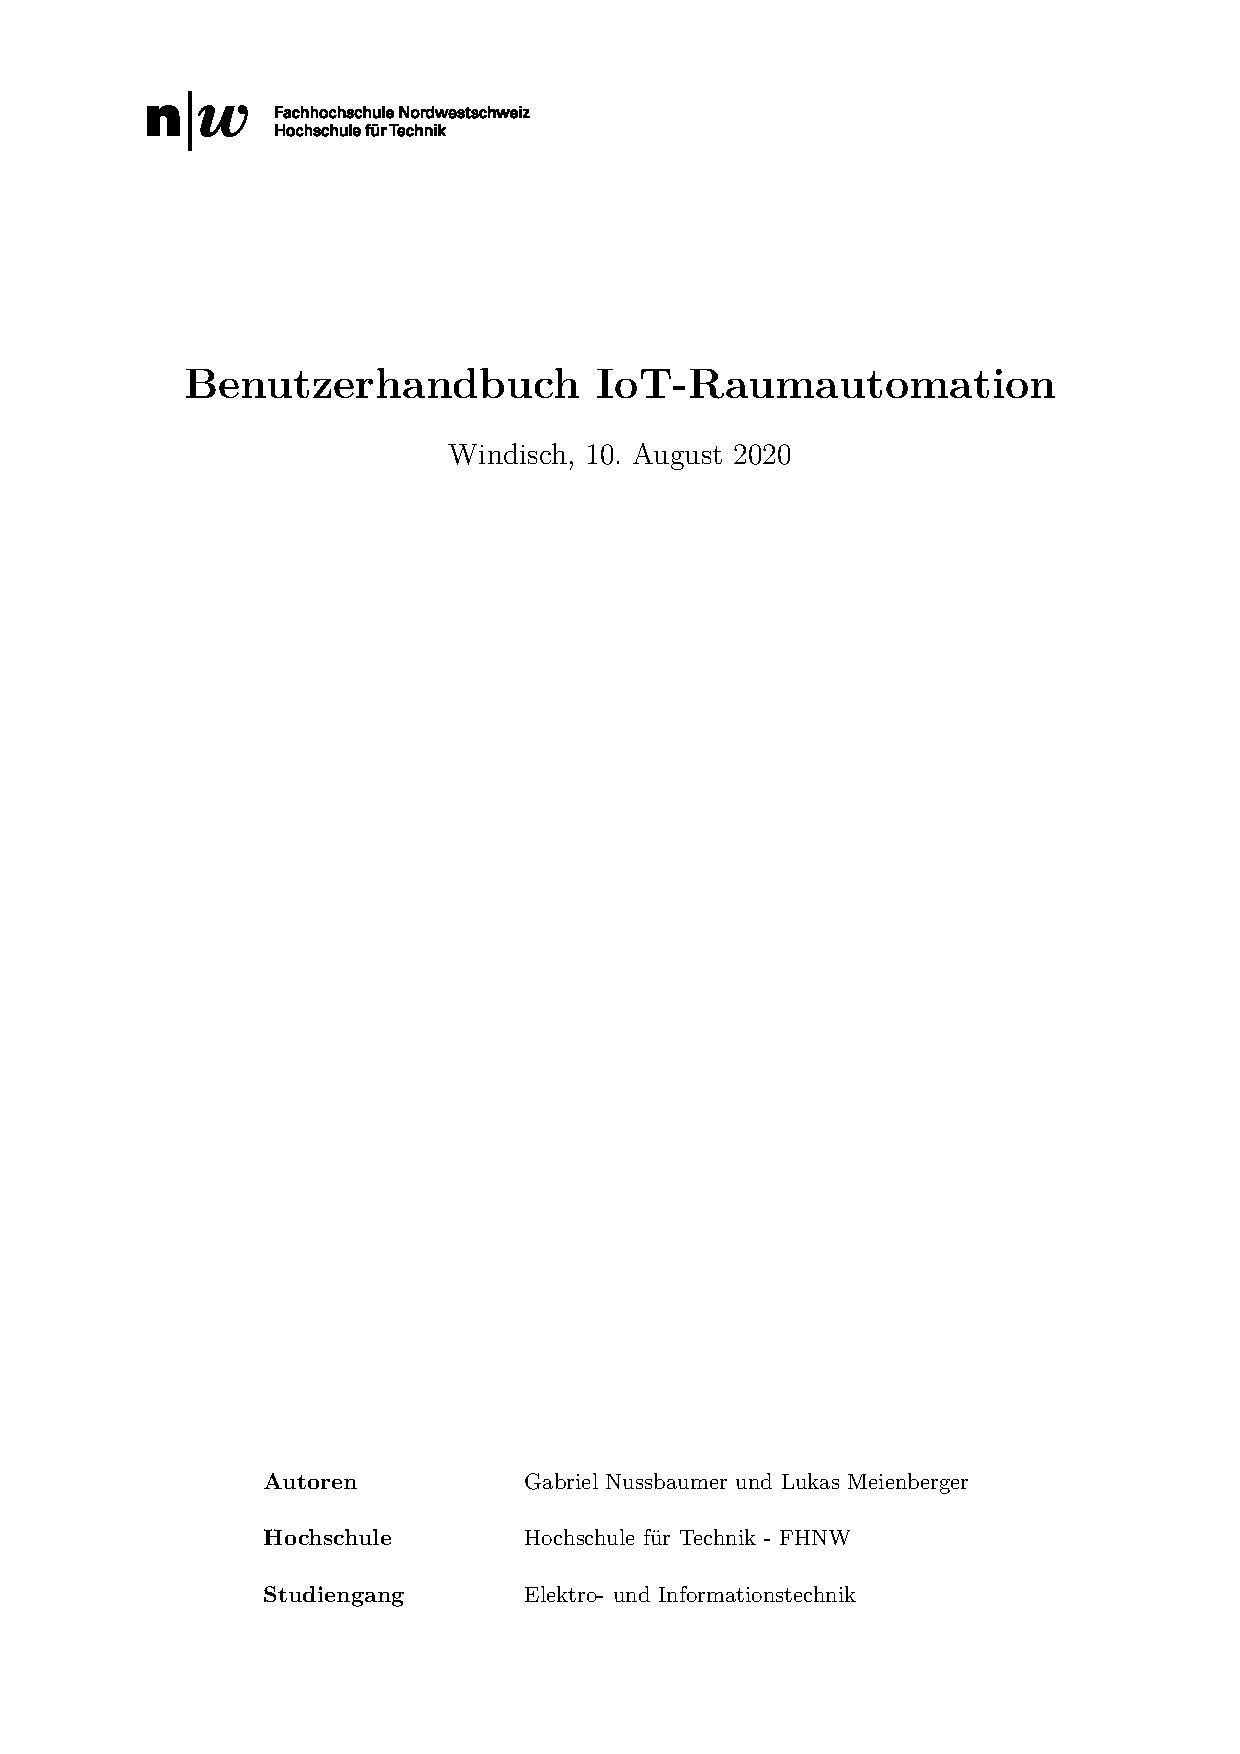
\includepdf[pages=-]{Benutzerhanndbuch.pdf} \newpage

%\includepdf[pages={1},nup=1x1,landscape=true,scale=0.85,offset=10 -40,pagecommand={\section{Eingefügte PDF-Tabelle}\label{app:Timetable}\thispagestyle{myheadings}}]{appendix/timeline_example.pdf} \newpage

%%Bei mehrseitigen Dokumenten die folgenden Seiten ohne Überschrift:
%\includepdf[pages={2-5},nup=1x1,landscape=true,scale=0.85,offset=0 -20,pagecommand={\thispagestyle{myheadings}}]{appendix/timeline_example.pdf} \newpage

\end{appendix}


%%---NOTES for DEBUG---------------------------------------------------------------------
%\ifdraft{%Do this only if mode=draft
%\usepackage{todonotes})
%\newpage
%\listoftodos[\section{Todo-Notes}]
%\clearpage
%}
%

\end{document}
